\begin{savequote}[8cm]
\textlatin{Neque porro quisquam est qui dolorem ipsum quia dolor sit amet, consectetur, adipisci velit...}

There is no one who loves pain itself, who seeks after it and wants to have it, simply because it is pain...
  \qauthor{--- Cicero's \textit{de Finibus Bonorum et Malorum}}
\end{savequote}

\chapter{\label{ch:35-nuint}Neutrino interactions} 
\minitoc

\section{nu-quark}
From QFT, write down Fenynman's rule explicitly

\section{nu-nucleon}
However, due to confinement and the relatively low energy, nu usually is interacting with the nucleon as a whole.
require form factors to paramterize the interaction with a nucleon.

\section{nu-nucleus}
Nuclear effect. 
The simplest case is for the relatively high energy nu, for wthich Impulse Approximation (IA) can be used.
Nu sees the nucleon as independent from other nucleons.
The interaction approaches the nu-nucleon interaction.

When the energy drops, IA is no longer valid and see the nucleus as a whole.
RPA correction is needed, beyond the scope of this thesis, will not ellaborate but interest reader can refer to REFXXX for more details.

  \subsection{Initial state}
  In addition to the different modes that the neutrino ineteract with the nucleus, the presence of the nuclear medium also affects the interaction.
  The nuclear effects manifest in two ways.
  Firstly, the nucleon in the interaction is in a bound state, i.e. it cannot have arbitrary energy and momentum like a free nucleon.
  Instead, the energy distribution of the nucleon is parameterised by the so-called Spectral Function (SF).
  The simplest form of SF is the Fermi Gas model, which treats the nucleons as freely moving Fermi gas.
  Hence, the nucleon momentum is filled up to the Fermi momentum, which is given as:
  <CHECK>
  \begin{equation}
      k_F = (3\pi^2 \rho/2)^{1/3},
  \end{equation}
  where $\rho$ is the nuclear density.
  <How is the fermi momentum determined?>
  This model oversimplifies the nuclear structure.
  A more realistic model is the local Fermi gas (LFG) model, which accounts for the varying nuclear density, leading to an SF of the form:
  (CHECK)
  \begin{equation}
      S(k, E) = \int \rho(\vec{r}) \delta(E - \sqrt{k^2 + m^2}) d^3r,
  \end{equation}
  where $m$ is the nucleon mass.

  Further improvement, such as the short-range correlation between nucleons that increases the high momentum fraction.
  There are also effective SFs. Fit to data?

  \subsection{FSI}
  \label{sec:nuint-fsi}
  The second nuclear effect is the Final State Interaction (FSI).
  Regardless of how the neutrino interacts with the nucleon, the interaction products are still inside the nucleus.
  They have to propagate through the nuclear medium to be detectable.
  The interactions with the nuclear medium are classified as FSI.
  They are more pronounced for hadrons than leptons, as the former are more likely to interact with the nuclear medium.
  There are several types of FSI, such as the elastic scattering, charge exchange, and absorption.
  \begin{enumerate}
      \item 
  CEX involves changing the charge of the participating particles; for example,
  \begin{equation}
      \pip + \n \rightarrow \piz + \p,
  \end{equation}
  or vice versa. This rescattering type is crucial for event topologies requiring the presence of a pion;  depending on the signal pion charge, CEX could migrate events between signal and background. 

  \item 
  INEL is the case where the nucleus is left in an excited state after the rescattering. This category only contains the situation where a single additional nucleon is emitted/knocked-out after rescattering. Since it does not affect the number of pions produced, it will not convert an event from a pionless topology to a pion-production topology. The effects on nucleons are two-fold. Firstly, it can alter the number of signal events within each event topology. If the inelastic rescattering leads to two low-momentum protons below the detection threshold as opposed to a high-momentum proton, this signal event will be discarded as no protons are observed. Secondly, INEL invariably changes the kinematics of the rescattering particle. Be it the leading proton or the leading pion, based on which the TKI observables are calculated, the TKI distribution shape will be affected. Hence, while $\ninel$ would affect all four data sets, $\piinel$ would only affect \ttkpip and \minpiz. 

  \item 
  ABS refers to the case where the particle undergoes an interaction so that it does not emerge as a final particle. For example, $\pi^+$ can interact with two or more nucleons, initially forming a baryon resonance that subsequently interacts with other nucleons, emitting multiple nucleons rather than pions. Hence, the $\pi^+$ would not emerge from the nucleus anymore.

  \item 
  PIPD happens for energetic particles where an extra pion emerges as a result of the rescattering, such as
  \begin{equation}
      \p + \p \rightarrow \p + \n + \pip.
  \end{equation}
  Such an interaction significantly alters the event topology. 

  \end{enumerate}


\section{\label{sec:1-intro}Introduction}

Neutrinos play a central role in advancing our understanding of physics and addressing fundamental inquiries in contemporary science. The Hyper-Kamiokande experiment~\cite{Hyper-Kamiokande:2018ofw} aims to conduct precise measurements of charge parity violation within the neutrino sector, a phenomenon believed to be closely linked to the observed matter-antimatter asymmetry in the universe. Similarly, the Deep Underground Neutrino Experiment (DUNE)~\cite{DUNE:2016hlj,DUNE:2015lol,DUNE:2016evb,DUNE:2016rla,DUNE:2021tad}  promises the same, in addition to elucidating the neutrino mass ordering. Whether seeking to ascertain Standard Model parameters or probing for exotic phenomena, significant enhancements in both theoretical frameworks and computational simulations of neutrino-nucleus interactions are imperative. As neutrinos interact mainly with nucleons inside the nucleus, the interaction is subject to nuclear effects, namely the nucleon initial state and final-state interactions (FSIs). These effects are difficult to calculate and can alter the final event topology by changing the number of final state pions with respect to the interactions on free nucleons. Notably, the neutrino flux at DUNE yields a comparable proportion of events with and without pions in the final state, highlighting the pressing need for a generator capable of accurately describing both event topologies.

The large data samples and superb imaging capabilities of modern neutrino experiments offer us a detailed new look at neutrino interaction physics.
Recently, the GENIE~\cite{Andreopoulos:2009rq, GENIE:2021npt} Collaboration has made substantial progress towards a global tuning using neutrino, charged lepton and hadron scattering data, in an attempt to integrate new experimental constraints with state-of-the-art theories and construct robust and comprehensive simulations of neutrino interactions with matter. 
Cross-experiment and cross-topology analyses are challenging tasks as each measurement features its unique selection criteria and various other  aspects, such as the neutrino flux. \genie has built an advanced tuning framework that enables the validation and tuning of comprehensive interaction models using an extensive curated database of measurements of neutrino, charged lepton and hadron scattering off nucleus and nuclei. So far, the non-resonant backgrounds~\cite{GENIE:2021zuu}, hadronization~\cite{GENIE:2021wox} and the quasielastic (QE) and 2-particle-2-hole (2p2h)  components~\cite{GENIE:2022qrc} of the neutrino-nucleus interaction have been tuned with $\nu_\mu$ and $\bar{\nu}_\mu$ charged-current (CC) pionless (0$\pi$) data from MiniBooNE, T2K and MINERvA. A partial tune was performed for each experiment, highlighting the neutrino energy dependence on the QE and 2p2h tuned cross sections. Even though post-tune predictions enhanced the data description for each experiment, the added degrees of freedom were not sufficient to fully describe all CC0$\pi$ data and exhibited tensions with some proton observables~\cite{GENIE:2022qrc}. More exclusive measurements result in additional model constraints. In addition, observables that are sensitive to targeted aspects of the complex dynamics of neutrino interactions are invaluable for model tuning. The transverse kinematic imbalance (TKI)~\cite{Lu:2015hea, Lu:2015tcr}, a final-state correlation between the CC lepton and the handronic system, is a good example since it is sensitive to the initial-state nuclear environment and hadronic FSI. Our next step is to incorporate TKI data from experiments where various exclusive topologies at different energies are considered. This marks the first combined tuning on TKI data with and without pions in the final states and serves as the starting point of a more comprehensive tuning effort in the energy region most relevant for future accelerator-based neutrino experiments.  


\section{TKI}
\label{sec:nuint-tki}

\begin{figure}[!htb] 	
    \centering 		
    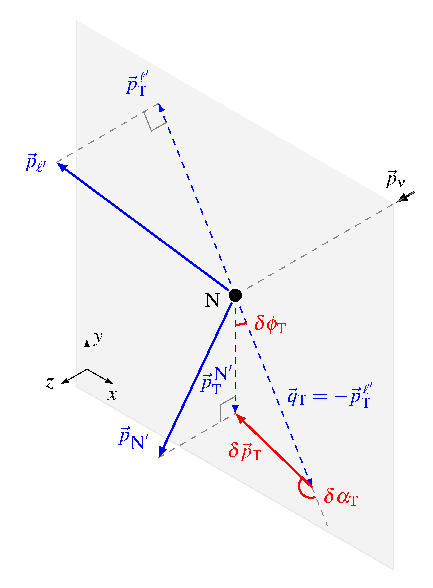
\includegraphics[width=0.35\textwidth]{figures/stki.eps}
    \caption{\label{fig:stki} Schematic illustration of the TKI variables. Diagram taken from Ref.~\cite{Lu:2015tcr}.} 
\end{figure}

The TKI variables are shown in Fig.~\ref{fig:stki}. They are cleverly constructed such that they are most sensitive to IS and FSI. 
In the simplest case, there are only two final particles after the neutrino-nucleon interaction, a muon and a proton. 
If the initial momentum of the struck nucleon has no component transverse to the neutrino's incoming direction, the products, i.e. the muon and the proton, should not have a net transverse component either, unless the struck nucleon has a non-zero initial transverse component or the final particles have undergone FSI.
Suppose there is no FSI, the net transverse component, $\dpt$, corresponds exactly to the magnitude of the transverse component of the struck nucleon, and the angle, $\dat$, represents the direction of the initial nucleon motion projected on the transverse plane. 
Assuming the nucleons are moving isotropically, the $\dat$ distribution should be flat. 
All current nuclear models do not have a preferential direction for initial nuclear motion, so it is only natural to assume the nucleons move in random directions. 
Thus, the deviation from flatness for $\dat$ can only be due to FSI, thereby making it an excellent probe for FSI. 
As for $\dpt$, it reflects the magnitude of the initial nucleon momentum transverse to the neutrino direction compounded by FSI. 
Furthermore, if the nucleus is assumed to be at rest and no other particles are knocked out other than the muon and the proton, the initial nucleon momentum, $\pn$, can also be derived following the steps outlined in \cite{pnpaper}. 
 

\section{TKI measurements}\label{sec:tki}


TKI is a methodology based on the conservation of momentum in neutrino interactions. In essence, it involves quantifying the imbalance between the observed transverse momentum of the final-state particles and the expected transverse momentum from neutrino interactions with free nucleons~\cite{Lu:2015hea, Lu:2015tcr}. This ``kinematic mismatch'' together with its longitudinal and three-dimensional variations~\cite{Furmanski:2016wqo, Lu:2019nmf}, and the derived asymmetry~\cite{Cai:2019jzk}, has been a crucial set of observables, establishing a pathway to extract valuable information about the participating particles and the underlying nuclear processes. Recent experimental results from neutrino experiments such as  T2K~\cite{T2K:2018rnz, T2K:2021naz}, MINERvA~\cite{MINERvA:2018hba, MINERvA:2019ope, MINERvA:2020anu, MINERvA:2021csy}, and MicroBooNE~\cite{MicroBooNE:2022emb, MicroBooNE:2023cmw, MicroBooNE:2023tzj, MicroBooNE:2023wzy, MicroBooNE:2024tmp}, as well as electron scattering experiments such as  CLAS~\cite{CLAS:2021neh}, highlight the efficacy of TKI. 

\begin{figure}[!htb] 	
    \centering 		
    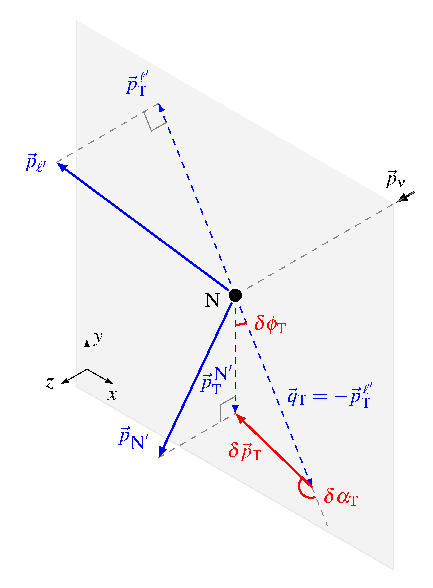
\includegraphics[width=0.35\textwidth]{figures/stki.eps}
    \caption{\label{fig:stki} Schematic illustration of the TKI variables. Diagram taken from Ref.~\cite{Lu:2015tcr}.} 
\end{figure}

In neutrino scattering off a free nucleon, the sum of the transverse components of the final products is expected to be zero, visualized through a back-to-back configuration between the final-state lepton and hadronic system in the  plane transverse to the neutrino direction. Hence, in a neutrino interaction with a nucleus, the transverse momentum imbalance, $\dpt$~\cite{Lu:2015tcr}, results from intranuclear dynamics, including Fermi motion and FSIs  as shown in Fig.~\ref{fig:stki}. The deviation from being back-to-back is quantified by the  coplanarity angle $\dphit$~\cite{Lu:2015tcr}, while the transverse boosting angle, $\dat$~\cite{Lu:2015tcr}, represents the direction of $\dpt$ within the transverse plane. Furthermore, analyzing the energy and longitudinal momentum budget~\cite{Furmanski:2016wqo, Lu:2019nmf} enables the conversion of $\dpt$ to the emulated (initial) nucleon momentum, $\pn$,  providing further insight into the Fermi motion; this conversion amounts to a correction on the order of $\mathcal{O}(20\%)$~\cite{Yang:2023dxk}. 
With one-body currents in the absence of FSIs, $\dat$ remains uniform (except for second-order effects, such as variations in the center-of-mass energy), given the isotropic nature of the initial nucleon motion. However, as the final products propagate through the nuclear medium, they experience FSIs, thereby disturbing the isotropy and the Fermi motion peak of the $\dat$ and $\pn$ ($\dpt$) distributions, respectively. Hence, $\dpt$ and $\pn$ elucidate the Fermi motion details, while $\dat$  characterizes the FSI strength---crucial for understanding medium effects in neutrino interactions. A notable advantage of these observables is their minimal dependence on neutrino energy~\cite{Lu:2015tcr}. Moreover, the double TKI variable, $\dptt$~\cite{Lu:2015hea}, is the projection of $\vecdpt$ along the axis perpendicular to the lepton scattering plane (hence ``double''). In addition to its use for extracting neutrino-hydrogen interactions~\cite{Lu:2015hea, Hamacher-Baumann:2020ogq}, it has also been applied to study nuclear effects in neutrino pion productions~\cite{MINERvA:2020anu, T2K:2021naz}. Its equivalent in pionless production, $\dptx$, has been proposed and studied together with its orthogonal companion, $\dpty$, in MINERvA~\cite{MINERvA:2019ope}. 